\documentclass[14pt]{extreport}
\usepackage{gost}

\begin{document}

\pagestyle{empty}
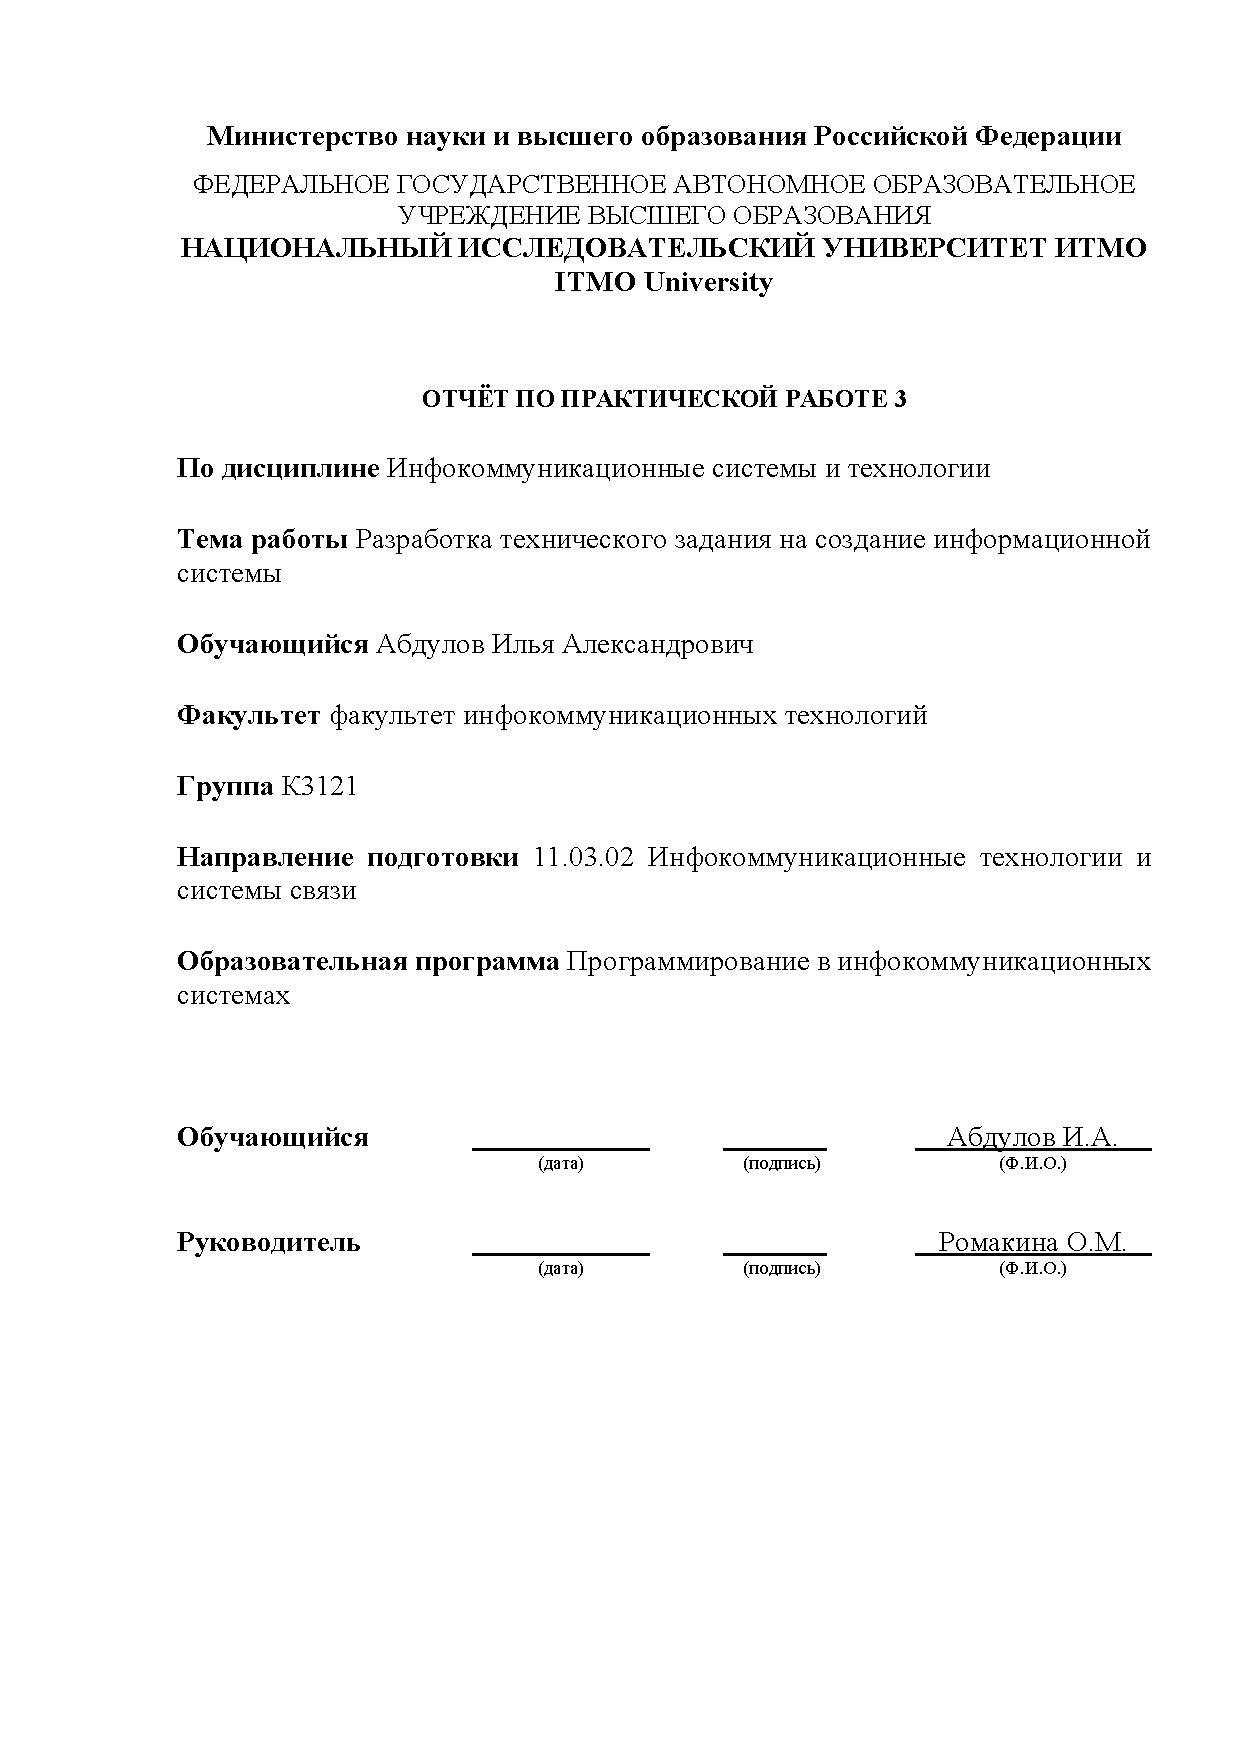
\includepdf{titulCourse.pdf}
\pagestyle{plain}

\tableofcontents

\intro

Опытному и уважающему себя программисту необходимо уметь реализовывать некоторые алгоритмы и структуры данных, знание которых облегчает решение многих повседневных задач, возникающих у типичного программиста.

Цель данной работы – ознакомление с алгоритмами поиска в глубину и ширину на языке программирования Python.

Данная работа представляет собой отчет о выполненных заданиях:
\begin{enumerate}
\item Написать программу, которая определяет, является ли введенная скобочная структура правильной.
\item Придумать и решить задачу для алгоритма поиска в глубину и для алгоритма поиска в ширину.
\item Написать алгоритм, который найдет выход из лабиринта.
\end{enumerate}

\chapter{Задание 1}

Определение правильности скобочной последовательности требует наличия счетчика, изначально равного нулю. Будем последовательно просматривать символы скобочной последовательности. Если символ – открывающая скобка, то к счетчику прибавим единицу, иначе прибавим минус единицу. Если в какой-либо момент времени счетчик станет отрицательным, это значит, что в тот момент времени количество закрывающих скобок превышало количество открывающих, то есть последовательность неверна. Если после прохода по символам всей строки счетчик равен нулю, то количество открывающих и закрывающих скобок совпадает, последовательность верна. 

Определение первого символа, нарушающего верность последовательности требует дополнительного счетчика который укажет индекс символа первой не закрытой скобки или первой скобки, не имеющей соответствующей открытой.

\begin{figure}[H]
\centerline{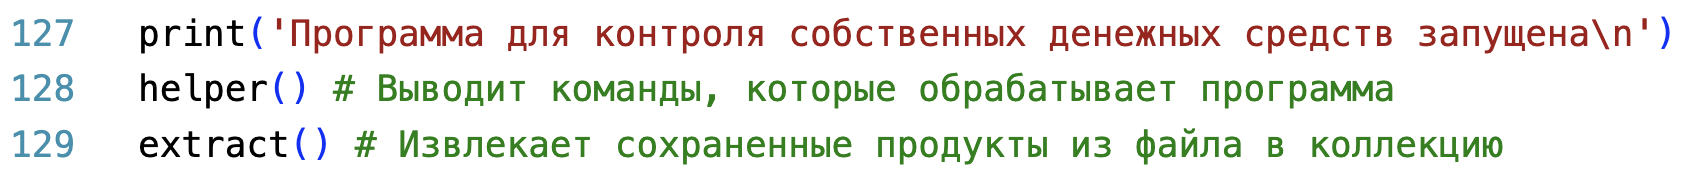
\includegraphics[width=1\linewidth]{Pic1.png}}
\caption{Код проверки скобочной последовательности на правильность}
\label{fig11}
\end{figure}

\begin{figure}[H]
\centerline{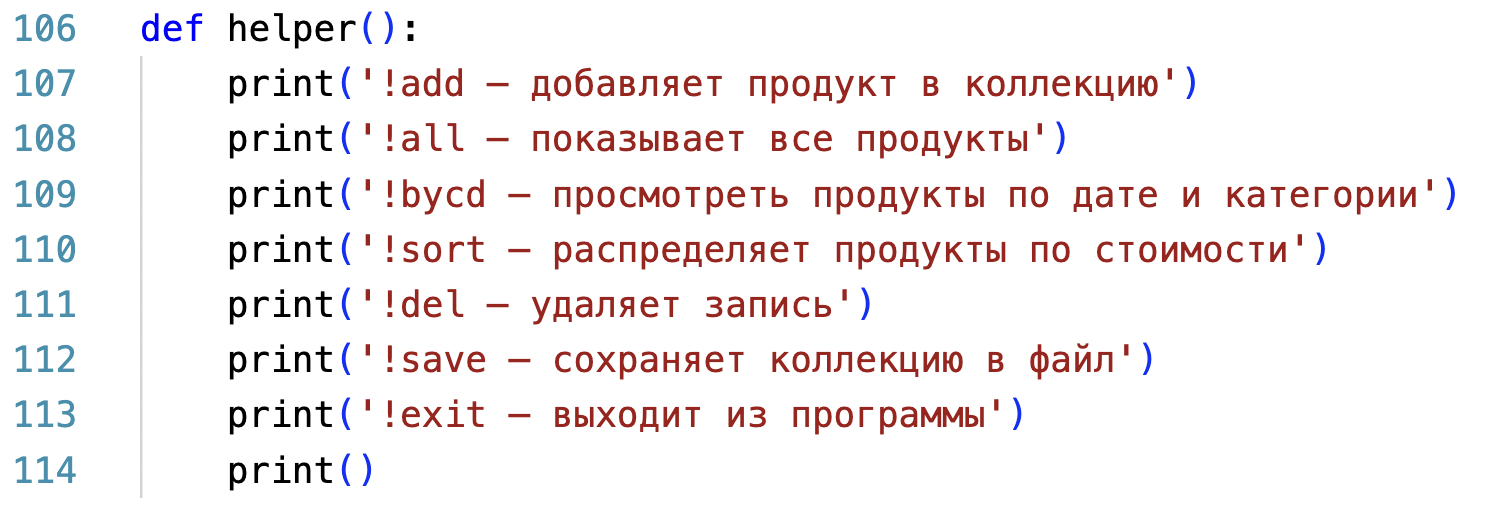
\includegraphics[width=0.8\linewidth]{Pic2.png}}
\caption{Пример работы кода по определению вида скобочной последовательности}
\label{fig12}
\end{figure}

Вывод: алгоритм определения вида скобочной последовательности требует внимательности в реализации и создается с использованием счетчика, который изменяется в зависимости от одного из двух видов символов, а именно открывающей и закрывающей скобки.

\chapter{Задание 2}

«Обход в глубину» или «Поиск в глубину» – это рекурсивный алгоритм поиска всех вершин графа или древовидной структуры данных. Цель алгоритма – пометить каждую вершину, как посещенную, избегая циклов. 

Для применения алгоритма поиска в глубину на практике была придумана следующая задача.

Дано дерево, необходимо найти его диаметр.

В первой строке два числа: 1. Количество вершин в дереве 2. Количество ребер.
Затем следует m пар чисел – ребра дерева.

Программа должна вывести диаметр дерева

Идея решения данной задачи проста: необходимо поиском в глубину найти два наибольших расстояния от корня дерева до его листьев. Диаметром дерева будет сумма двух наибольших расстояний.

\begin{figure}[H]
\centerline{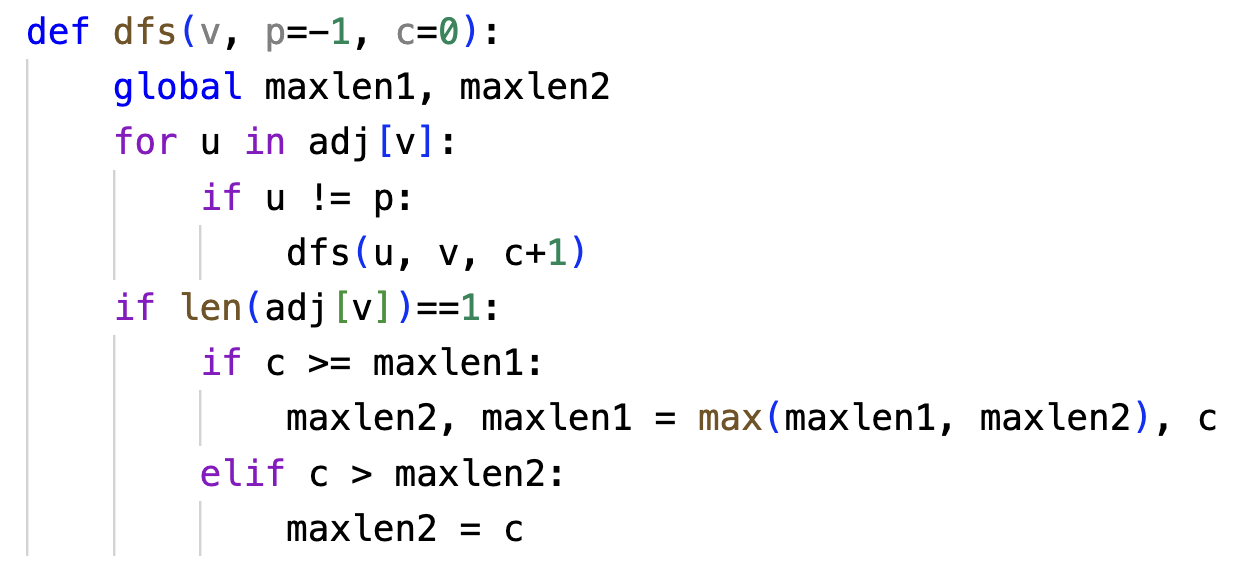
\includegraphics[width=1\linewidth]{Pic3.png}}
\caption{Код функции поиска в глубину при решении задачи}
\label{fig13}
\end{figure}

\begin{figure}[H]
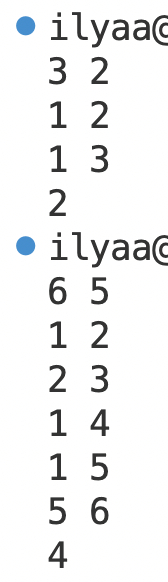
\includegraphics[width=0.1\linewidth]{Pic4.png}
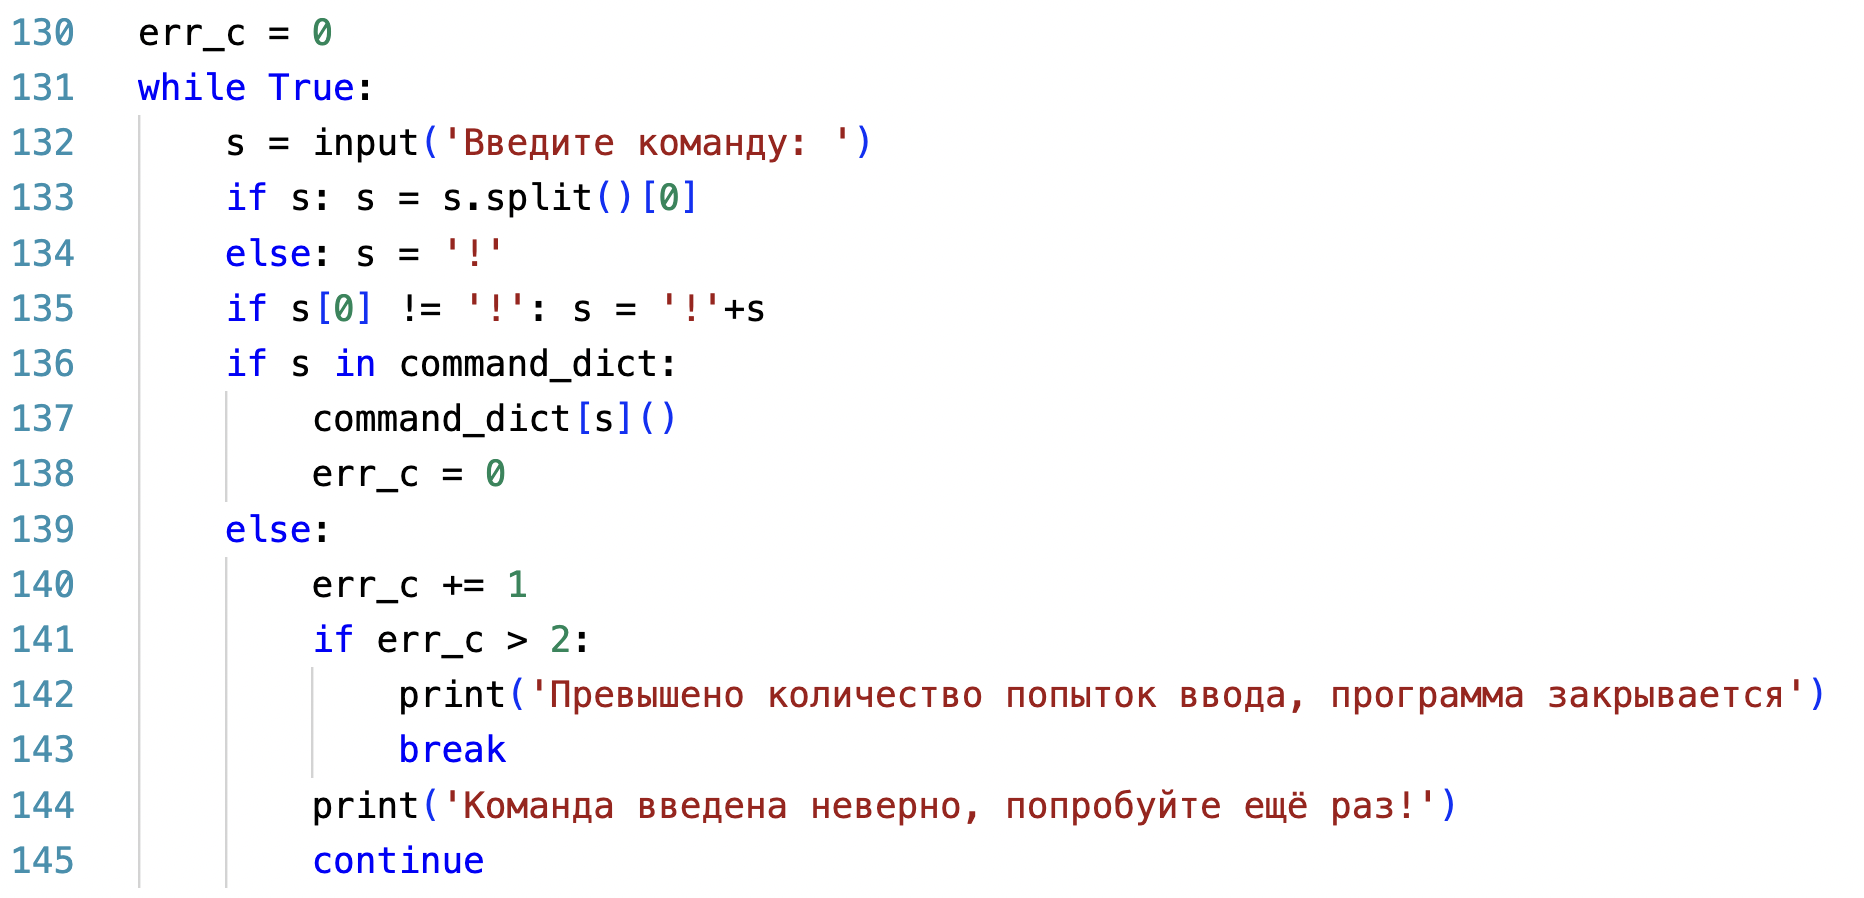
\includegraphics[width=0.8\linewidth]{Pic5.png}
\caption{Пример программы с применением поиска в глубину}
\label{fig14}
\end{figure}

Алгоритм поиска в ширину (англ. breadth-first search, BFS) позволяет найти кратчайшие пути из одной вершины невзвешенного графа до всех остальных вершин. Под кратчайшим путем подразумевается путь, содержащий наименьшее число ребер.

Для применения алгоритма поиска в ширину на практике была придумана следующая задача.

Дано дерево, необходимо найти эксцентриситет вершины.

В первой строке три числа: 1. Количество вершин в дереве 2. Количество ребер 3. Вершина.
Затем следует m пар чисел – ребра дерева.

Требуется вывести эксцентриситет введенной вершины

Идея решения данной задачи такова: считаем, что дистанция до введенной вершины равна нулю, будем считать расстоянием до вершин дерева сумму дистанции родительской вершины плюс один, посещая только ранее не посещенные вершины. Тогда максимальная из дистанций посещенных вершин будет искомым эксцентриситетом. 

\begin{figure}[H]
\centerline{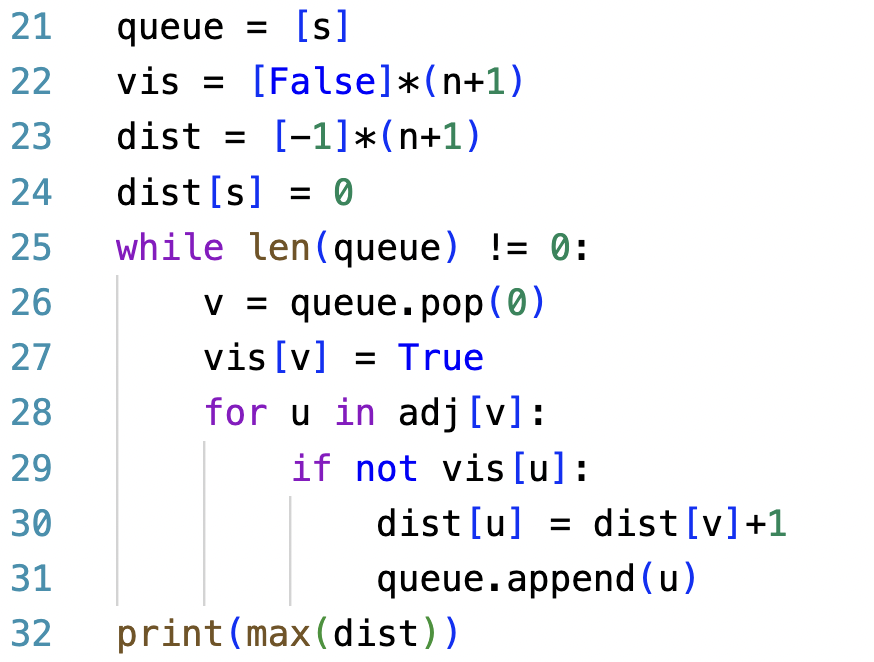
\includegraphics[width=1\linewidth]{Pic6.png}}
\caption{Код функции поиска в ширину при решении задачи}
\label{fig17}
\end{figure}

\begin{figure}[H]
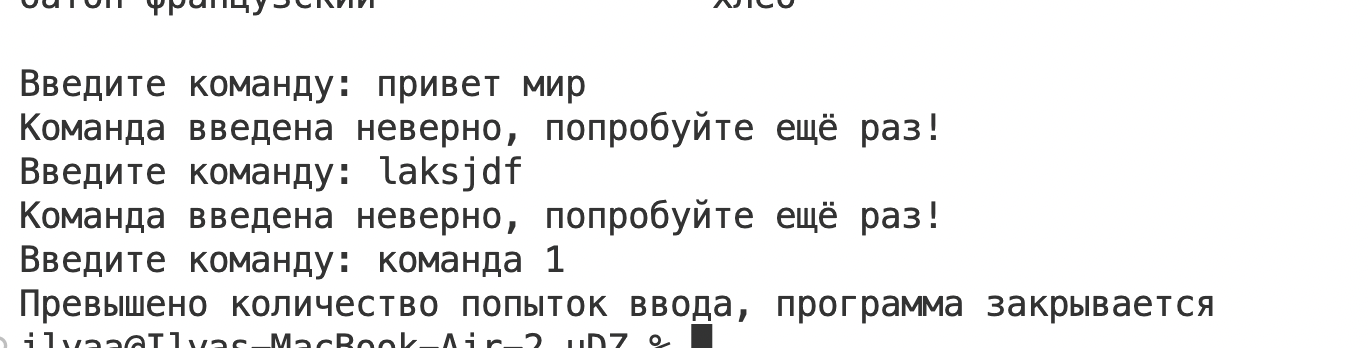
\includegraphics[width=0.1\linewidth]{Pic7.png}
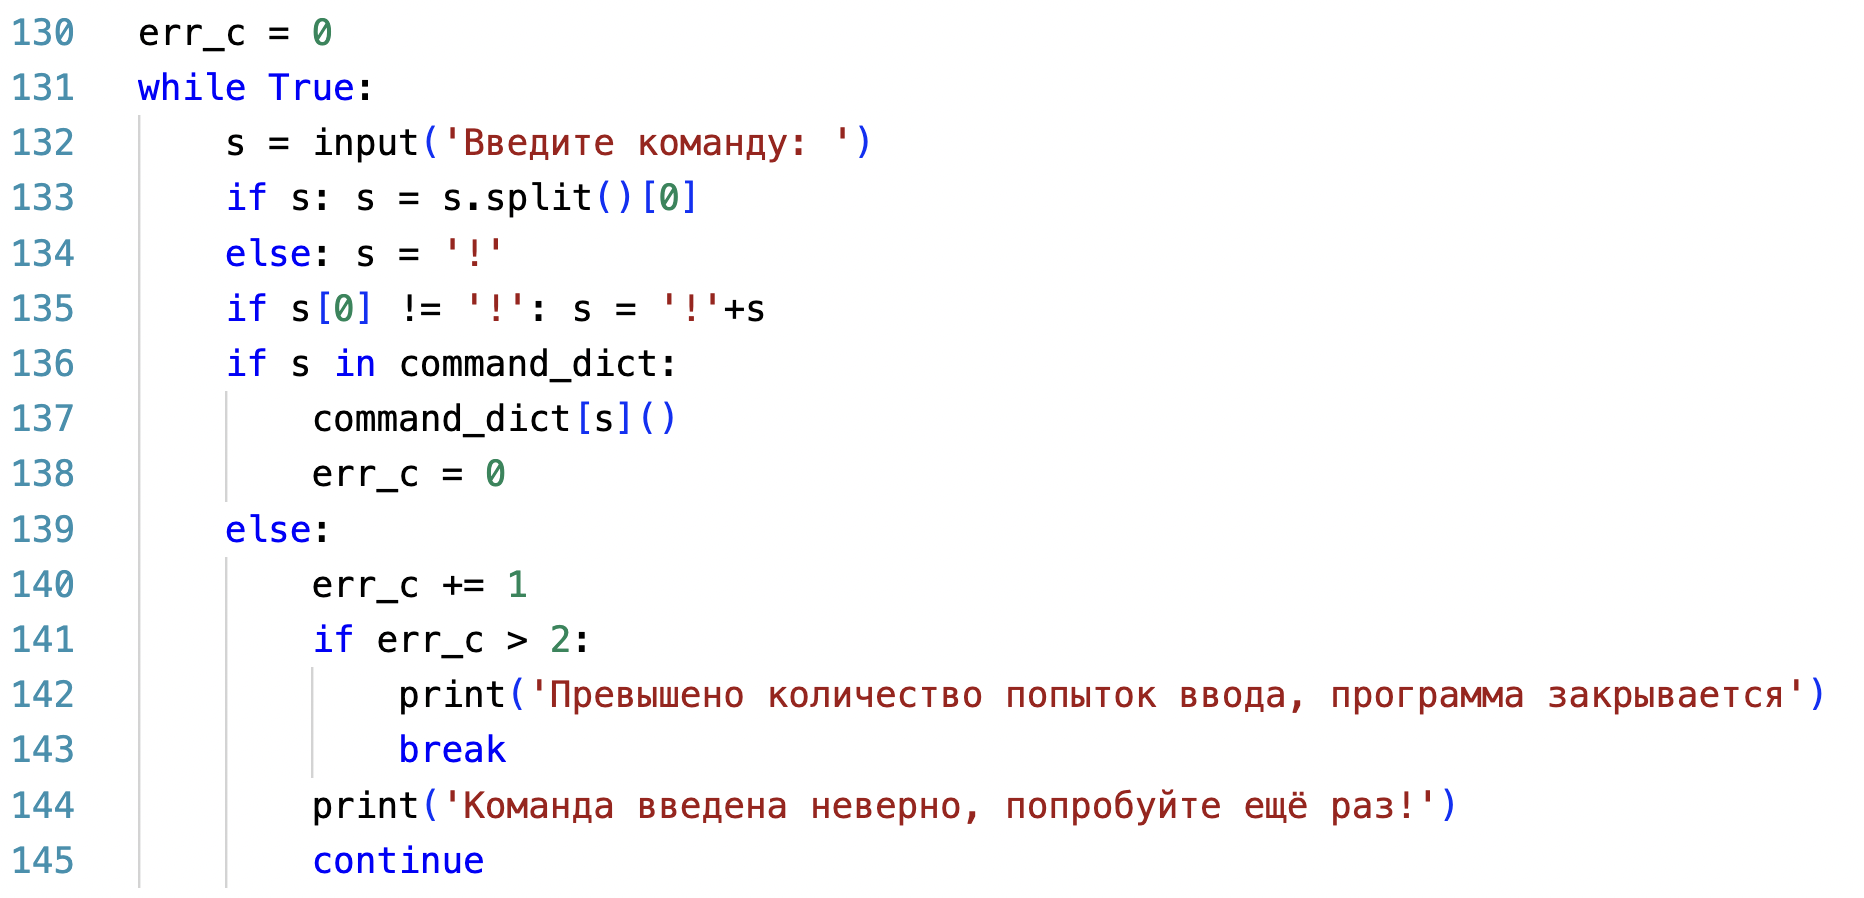
\includegraphics[width=0.8\linewidth]{Pic5.png}
\caption{Пример программы с применением поиска в ширину}
\label{fig18}
\end{figure}

Вывод: алгоритмы поиска в глубину и ширину отличаются программной реализацией, но могут быть оба применены для решения одной и той же задачи.

\chapter{Задание 3}

Для решения задачи с поиском выхода из лабиринта, в котором 0 – это проход, а 1 – это стена, был выбран алгоритм поиска в ширину, потому что его нерекурсивную реализация в данной программе будет проще модифицировать.

В структуре данных очередь в рамках данной программы будут находится пары индексов матрицы. Добавляться в очередь будут не посещенные нулевые клетки поля лабиринта слева, справа, снизу или сверху от извлеченной из очереди клетки. Как только в очереди появится пара индексов таких, что индекс находится на правой границе лабиринта, цикл поиска в ширину завершит работу.

\begin{figure}[H]
\centerline{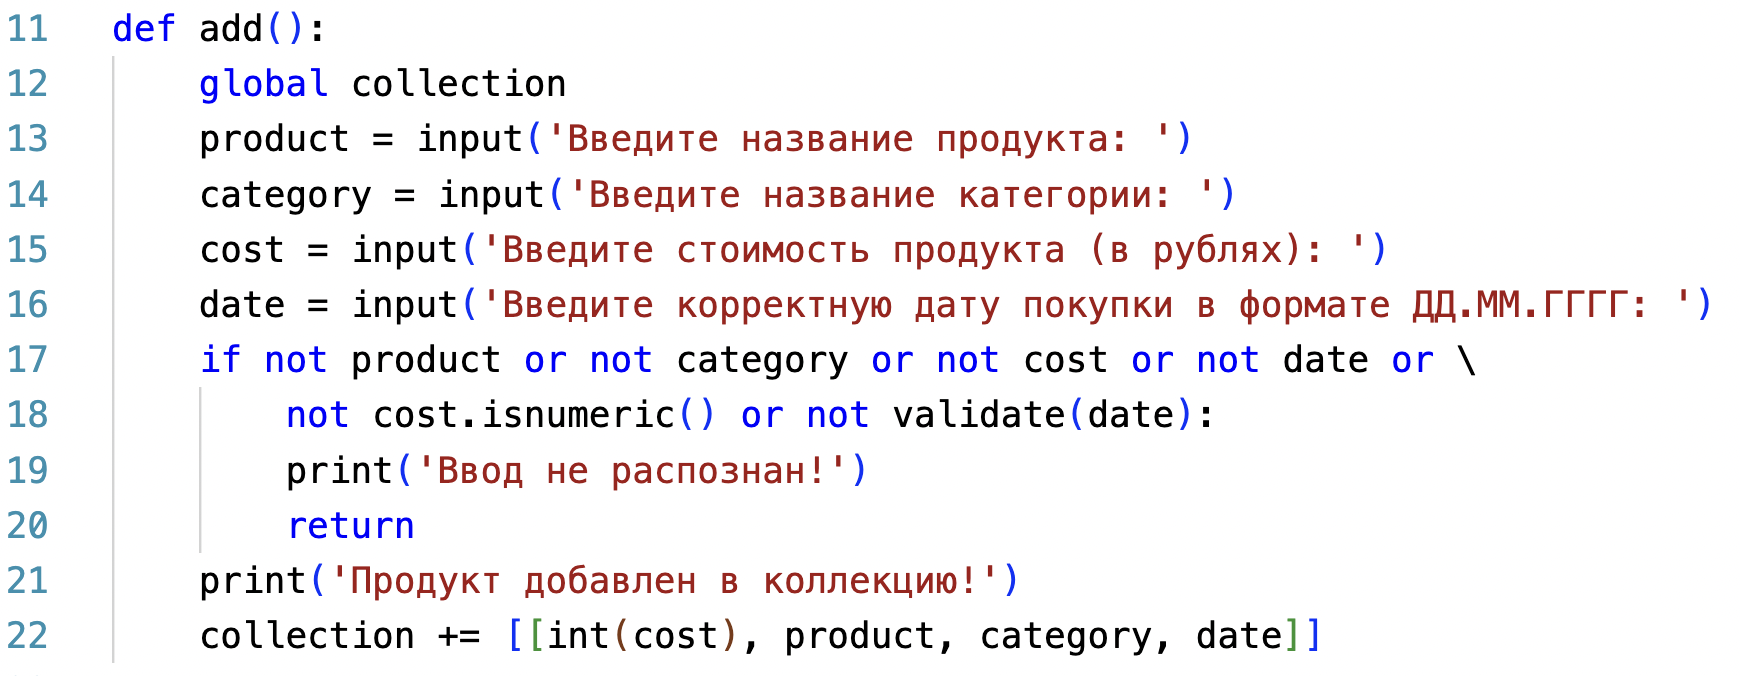
\includegraphics[width=1\linewidth]{Pic8.png}}
\caption{Код функции поиска в ширину для данной задачи}
\label{fig19}
\end{figure}

\begin{figure}[H]
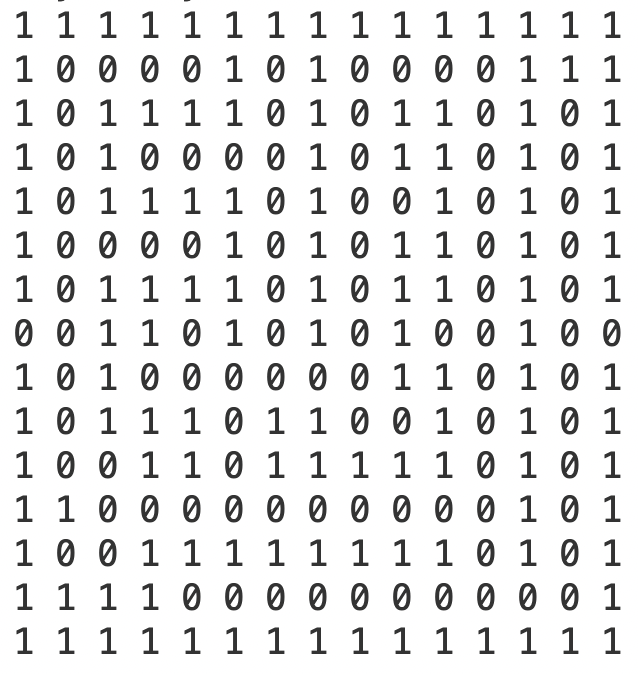
\includegraphics[width=0.5\linewidth]{Pic9.png}
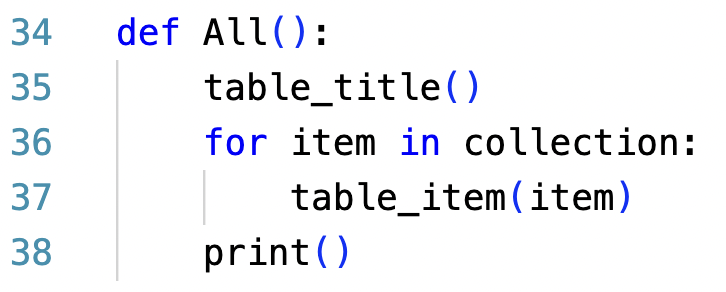
\includegraphics[width=0.5\linewidth]{Pic10.png}
\caption{Пример работы программы для заданной в условии задачи матрицы}
\label{fig20}
\end{figure}

\conclusions

Таким образом, для каждой задачи была написана программа на языке программирования Python. Были изучены алгоритмы DFS и BFS, которые важны в теории графов и используются для решения многих интересных задач, варианты которых представлены в отчете. Для каждого алгоритма приведена программная реализация.

Все программы можно найти на репозитории в GitHub\cite{bib1}.

\newpage
\begin{thebibliography}{99}

\bibitem{bib1}GitHub [Электронный ресурс]: \url{https://github.com/estle/itmo-uni/tree/main/sem1/ADS/lab5} (дата обращения 15.12.2022).

\end{thebibliography}

\end{document}
